\section{System Design and Implementation}

\subsection{System Overview}

The system consists of three major components. These are:

\begin{enumerate}
    \item an Arduino with sensors,
    \item a Raspberry Pi connected to the Arduino, and
    \item a laptop computer serving as «the Cloud».
\end{enumerate}

The sensors (SCD30, potentiometer, push button) take their input from the environment and the user, respectively. A small program on the Arduino collects the data every other second, and forwards it over a simple UART protocol via the USB port to the Raspberry Pi.

On the Raspberry Pi, there are running two processes: First, the \textit{Data Collector} receives the measurements from the Arduino via the USB port, and converts them to a dictionary. Second, the \textit{Data Forwarder} waits for incoming measurements in the form of a dictionary, converts it into a JSON structure, and forwards that to «the Cloud» using an InfluxDB client. On «the Cloud», the data is gathered in an InfluxDB and visualized in Grafana.

\subsection{System Architecture}

Figure \imgref{fig:architecture} shows the overall system architecture.

\begin{figure}
	\centering
	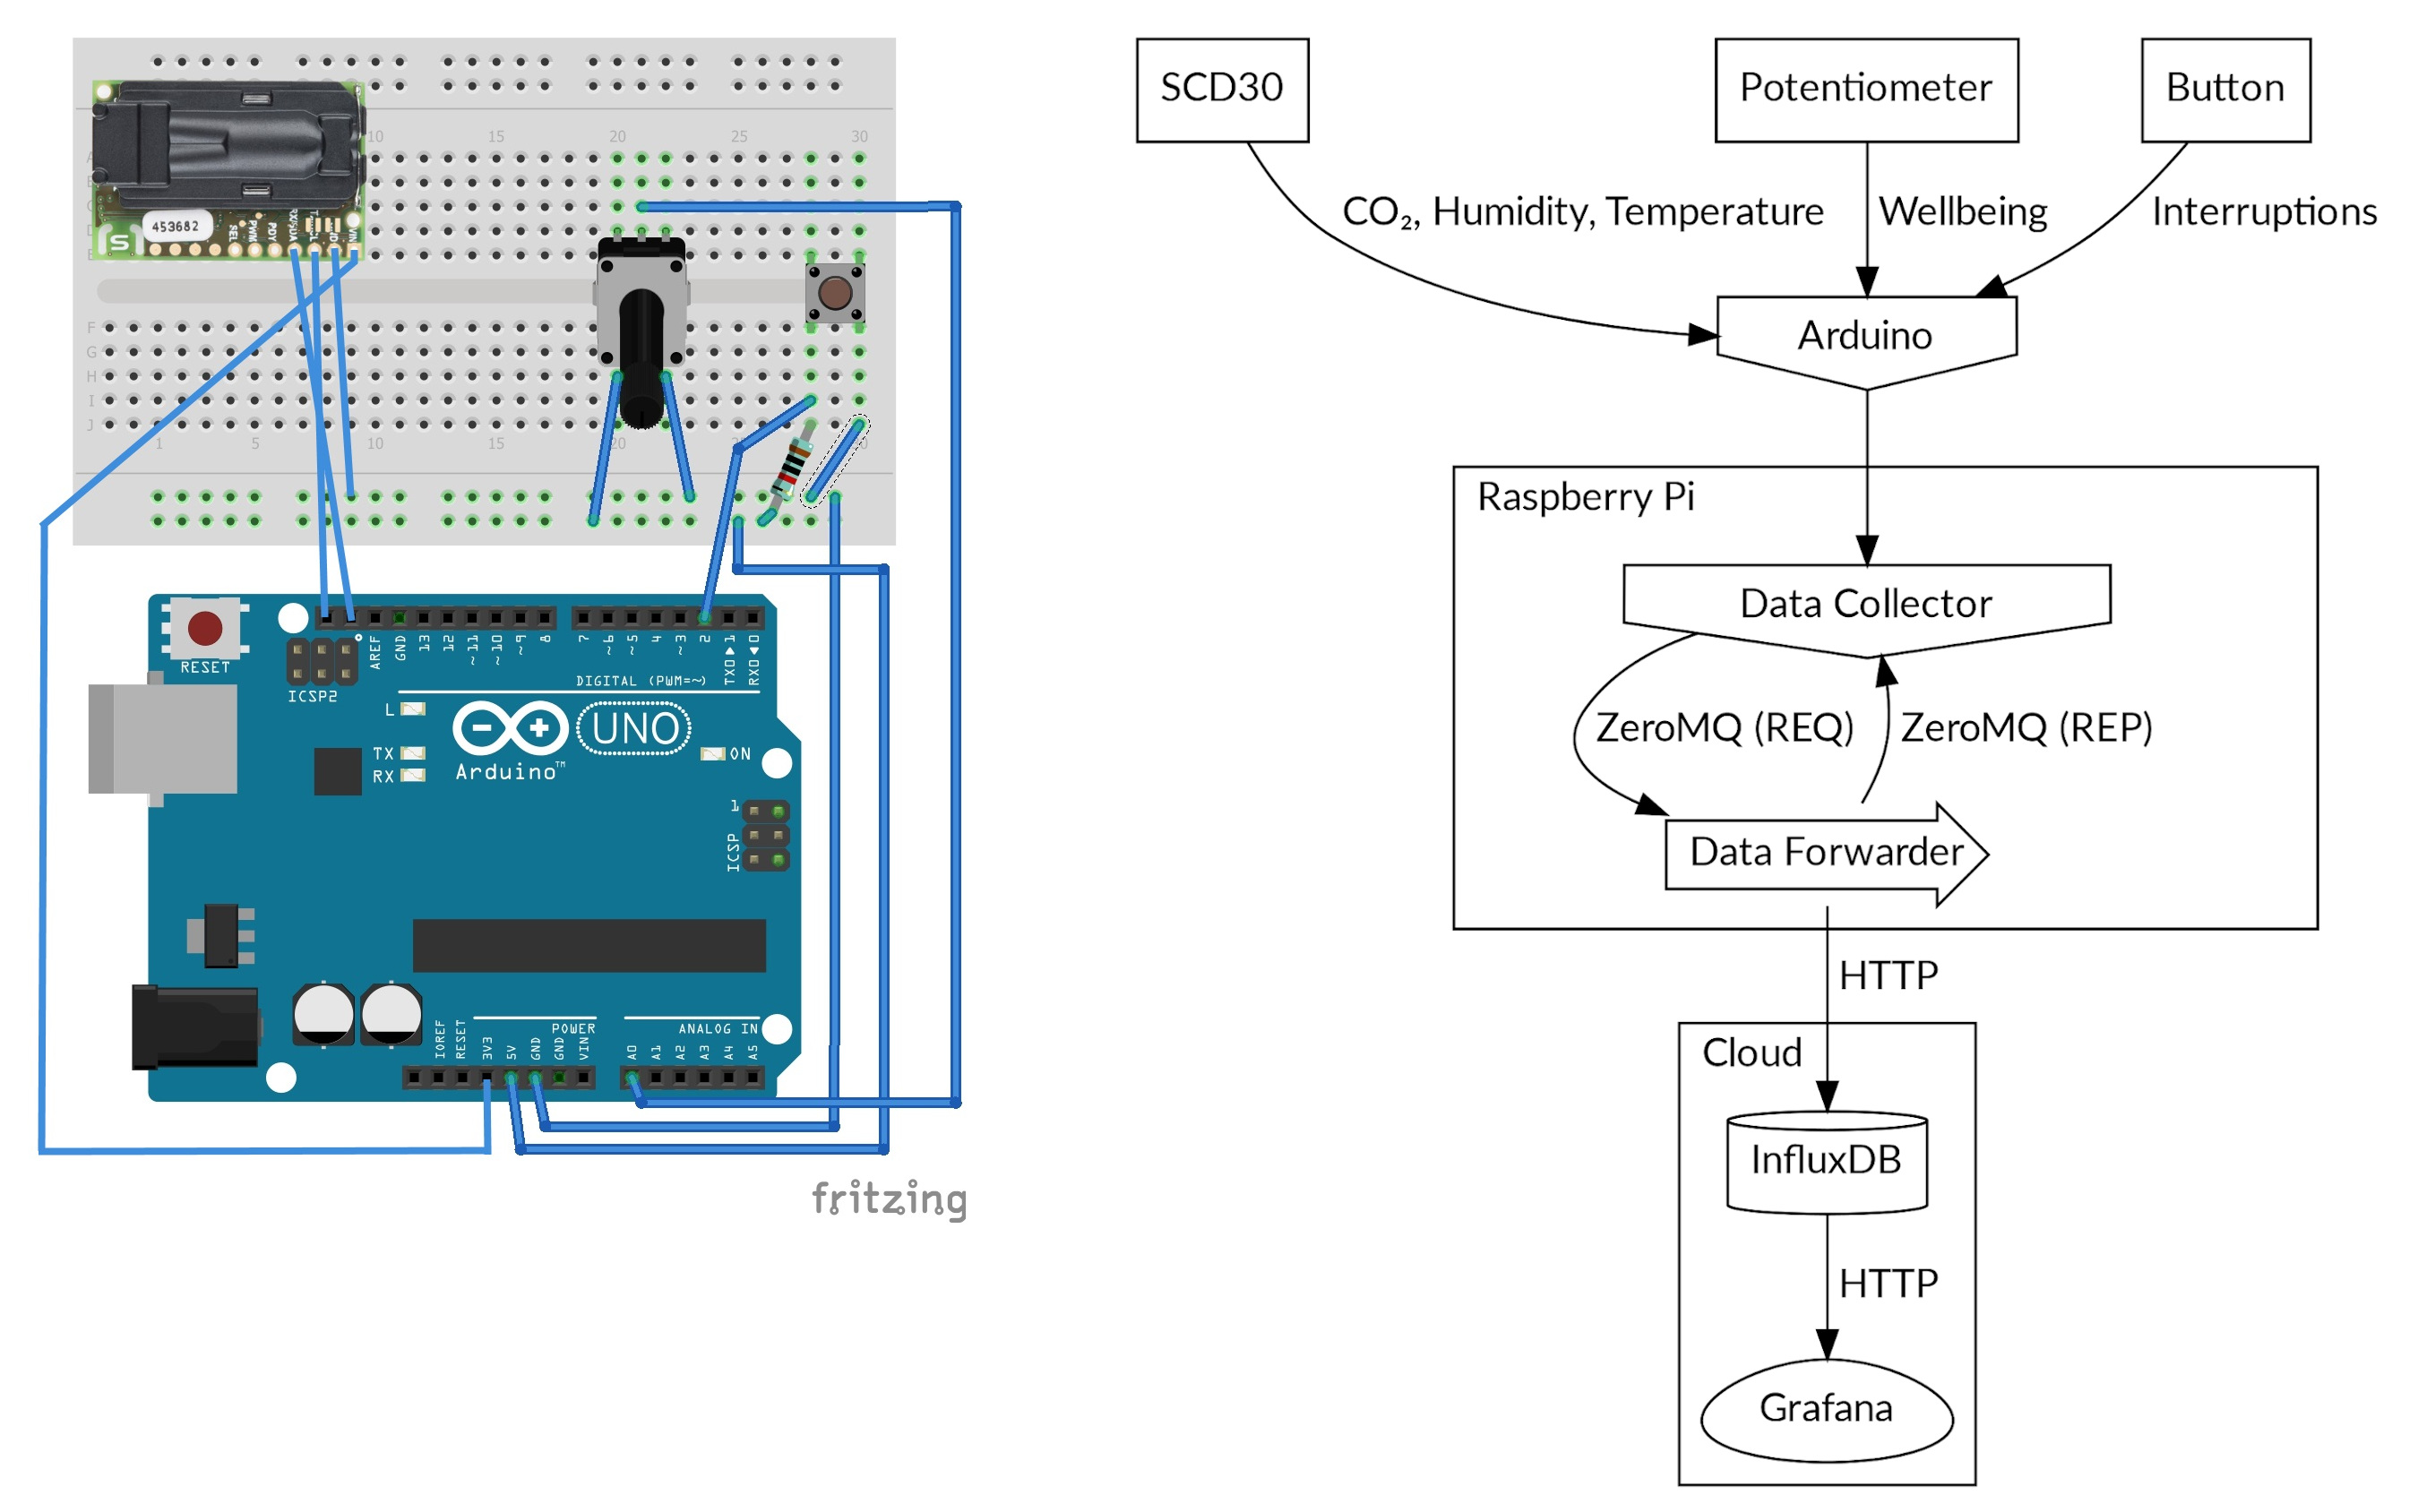
\includegraphics[width=\linewidth]{Architecture_Arduino.jpg}
	\caption{Model of Arduino circuit board and overall system architecture}
	\label{fig:architecture}
\end{figure}

\subsection{Software Architecture: Layers \& Modules}

The Arduino and the Raspberry Pi communicate over a simple string-based protocol. The payloads consist of key-value pairs:

\begin{verbatim}
key=value,key=value,key=value
\end{verbatim}

The following payload shows measurements for CO₂, temperature, humidity, interruption, and well-being.

\begin{verbatim}
co2=1024,temp=25.49,humid=47.39,interrupt=0,wellbeing=7
\end{verbatim}

The SCD30 produces the three first measurements at least every two seconds. This time is spent actively waiting in the interruption detection loop for the button to be pressed. If the button was pressed during that period, 1 is reported, and 0 otherwise. This approach does not require any concurrency on the Arduino side, and only allows for an interruption being detected every other second, which is considered to be sufficient.

The string payload is terminated by a newline character. When the reading Data Collector process on the Raspberry Pi starts, all the characters until the first newline character are discarded, since the process might be ready in the middle of a transmission. The key-value string is converted into a Python dictionary by applying two split operations on it, first using the comma, second using the equal sign. The created dictionary is «pickled» (Python jargon), i.e. serialized into a list of bytes, and sent over to the Data Forwarder.

The two processes ‒ Data Collector and Data Forwarder ‒ are connected through a ZeroMQ socket, using a simple request-response protocol. This protocol could easily be switched to a publish-subscribe pattern, which would allow for multiple Data Collectors to report to one or many Data Forwarders, which in turn would allow to track the inputs from multiple Arduino devices in a multitude of data base backends.

The Data Forwarder «unpickles» (Python jargon again) the received bytes back into a dictionary, which is then converted to a JSON structure. This JSON structure is sent to the InfluxDB on «the Cloud» using HTTP. Grafana is used to visualize the time series stored on Influx DB.

\subsection{System Implementation, Functional Software Architecture}

The architecture described allows for a lot of flexibility. The processes on the Raspberry Pi are unaware of any semantics, they only process data as key-value pairs in various formats. If a different Arduino with different sensors is plugged into the Raspberry Pi on one side, then the visualizations on Grafana just needs to be configured to deal with the new table. All the knowledge required on both sides is the name of the key that is transmitted from the Arduino to the Raspberry Pi, and that will serve as the table name in InfluxDB.

On the Arduino, the \texttt{Wire} library is used for serial data transmission, as well as the header \texttt{SparkFun\_SCD30\_Arduino\_Library.h} used for the sensor SCD30. Other configurations of the Arduino use the \texttt{Adafruit\_BME280}.

The libraries used on the Raspberry Pi are \texttt{zmq} (ZeroMQ), \texttt{InfluxDBClient} (InfluxDB), in addition to the Python standard library.
